\documentclass{../notatki}

\title{Mechanika Ogólna}

\usetikzlibrary{calc}

\begin{document}

\tableofcontents

\setcounter{section}{-1}

\section{Wstęp}

\subsection{Literatura}

\begin{itemize}
  \item D. H., R. R., Jearl Walker "Fundamentals of Physics"
  \item R. Shankar "Fundamentals of Physics"
\end{itemize}

\subsection{Całki}

Całki to operacje odwrotne do pochodnych. Dla funkcji $f(x)$ całka oznaczona
to pole pod wykresem funkcji $f(x)$ na przedziale $[a, b]$. Pozwalają nam
obliczyć pole pod krzywą, a także sumę nieskończenie wielu wartości funkcji.

\begin{figure*}[ht]
  \centering
  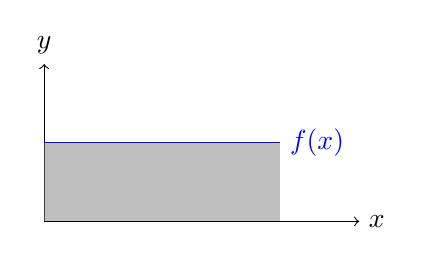
\begin{tikzpicture}
    \draw[->] (0, 0) -- (4, 0) node[right] {$x$};
    \draw[->] (0, 0) -- (0, 2) node[above] {$y$};
    \draw[domain=0:3, smooth, variable=\x, blue] plot
    ({\x}, {1}) node[right] {$f(x)$};
    \fill[fill=gray, fill opacity=0.5] (0, 0) -- (0, 1) -- (3, 1) --
    (3, 0) -- cycle;
  \end{tikzpicture}
  \caption{Całka oznaczona funkcji $f(x)$ na przedziale $[0, 3]$}
\end{figure*}

$$
f(x) = 1, \quad \int_0^3 f(x) dx = \int_0^3 3 dx =\left[x\right]^3_0 = 3 - 0 = 3
$$
albo, o wiele prościej:

$$
\int_0^3 f(x) dx = 3 \cdot 1 = 3
$$
Naturalnie nie zawsze możemy obliczyć całkę oznaczoną w ten sposób. Wtedy
musimy posłużyć się bardziej zaawansowanymi metodami.
Aby zademonstrować zastosowanie całek wyobraźmy sobie ciało co się porusza
ciągle przyspieszając w jednym kierunku. $a(t) = t^2$. Jeśli chcielibyśmy
obliczyć prędkość ciała w chwili $t = 3$ to chcemy dodać wszystkie
przyspieszenia
jakie ciało doświadczyło do tej chwili. Wtedy mamy:

\begin{figure*}[ht]
  \centering
  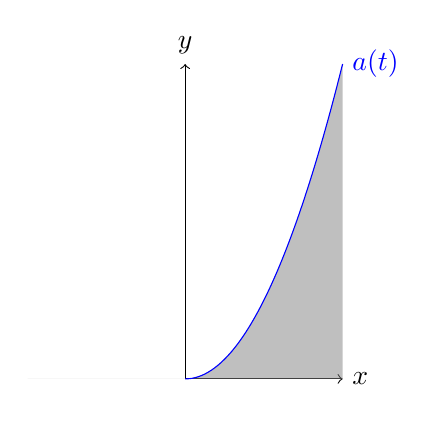
\begin{tikzpicture}
    \draw[->] (0, 0) -- (2, 0) node[right] {$x$};
    \draw[->] (0, 0) -- (0, 4) node[above] {$y$};

    \fill [gray, fill opacity=0.5, domain=0:2, variable=\x]
    (-2, 0)
    -- plot ({\x}, {\x*\x})
    -- (2, 0)
    -- cycle;
    \draw[domain=0:2, smooth, variable=\t, blue] plot
    ({\t}, {\t * \t}) node[right] {$a(t)$};
  \end{tikzpicture}
  \caption{Całka oznaczona $a(t)$ na przedziale $[0, 3]$}
\end{figure*}

$$
v(t) = \int^3_0 a(t) dt = \int^3_0 t^2 dt = \left[\frac{t^3}{3}\right]^3_0 = 9
$$

\section{Kinematyka}

Kinematyka to nauka o ruchu ciał.

\subsection{Wielkości średnie i chwilowe}

Wielkości średnie, to takie których doświadcza ciało w czasie $\Delta t$.
Z kolei wielkości chwilowe, to takie które opisują ciało w danym momencie.
Idealnym przykładem jest prędkość. $v(t)$ to prędkość chwilowa, a $v_{\Delta t}$
to prędkość średnia.

\subsection{Ruch}

Ruch ciała można opisać przy pomocy dwóch wielkości. Prędkości chwilowej ($v$),
oraz przyspieszenia chwilowego ($a$).

$$
v = \frac{\Delta s}{\Delta t}
$$

$$
v(t) = v_0 + a(t) \cdot t = v_0 + \int a(t) dt
$$

$$
a = \frac{\Delta v}{\Delta t} = v'
$$

Dla pozycji ciała $x$ mamy:

$$
x(t) = x_0 + v_0t + \frac{1}{2}a t^2 = x_0 + \int v(t) dt
$$

\subsection{Ruch w wielu wymiarach}

Aby opisać ruch w $n \in \mathbb{N}$ wymiarach, potrzebujemy po prostu $n$
wymiarowych wektorów. Dla ruchu w dwóch wymiarach mamy:

\begin{figure*}[ht]
  \centering
  \begin{tikzpicture}
    \draw [->] (0,0) -- (4.0,0) node [below right] {$x$};
    \draw [->] (0,0) -- (0,4.0) node [above right] {$y$};
    \coordinate (A) at (0.5,1);
    \coordinate (B) at (3,3);
    \draw [->] (A) -- (B) node [midway, above] {$\vec{v}$};
    \draw [dashed] (A) -- (3,1) node [midway, below] {$\vec{v}_x$};
    \draw [dashed] (3,1) -- (3,3) node [midway, right] {$\vec{v}_y$};
    % draw the angle
    \draw[draw=blue] (A) ++(0:10mm) arc (0:39:10mm) node[midway,
    left]{$\alpha$};
  \end{tikzpicture}
  \caption{Dekonstrukcja prędkości na składowe}
\end{figure*}

$$
\vec{v}_x = |\vec{v}| \cos \alpha, \quad \vec{v}_y = |\vec{v}| \sin \alpha
$$

\subsection{Ruch po okręgu}

Dla ruchu po okręgu mamy:

$$
a = \frac{v^2}{r}
$$

\section{Siły}

Miara wielkości oddziaływania ciał na siebie to siła.

$$
F = m \cdot a
$$
Dla siły grawitacyjnej działającej na ciało o masie $m$ pod kątem
$\alpha$ do osi $x$ mamy:

$$
F_g = m \cdot g \cdot \sin \alpha
$$

\subsection{Prawa Newtona}

\begin{enumerate}
  \item Ciało pozostaje w spoczynku lub porusza się ruchem jednostajnym
    prostoliniowym, jeżeli na nie nie działa żadna siła. $\sum F = 0
    \rightarrow \Delta v = 0$.
  \item Jeżeli na ciało działa siła, to ciało porusza się z przyspieszeniem
    proporcjonalnym do siły i odwrotnie proporcjonalnym do masy ciała.
  \item Jeżeli ciało działa na inne ciało siłą, to drugie ciało działa na
    pierwsze siłą o tej samej wartości, ale przeciwnie skierowaną.
\end{enumerate}

\subsection{Ciążenie powszechne}

Każda para ciał we wszechświecie oddziałuje na siebie siłą grawitacyjną.

$$
F_g = G \cdot \frac{m_1 \cdot m_2}{r^2}
$$
gdzie $G$ to stała grawitacyjna, $m_1$ i $m_2$ to masy ciał, a $r$ to odległość
między nimi.

\subsection{Tarcie}

Tarcie to siła przeciwna kierunku ruchu ciała. Wyróżniamy tarcie statyczne i
kinetyczne. Tarcie statyczne oddziałuje na ciała gdy te nie poruszają się, a
tarcie kinetyczne gdy ciała poruszają się. W pewnym sensie tarcie statyczne
określa siłę potrzebną do wzruszenia ciała, a tarcie kinetyczne to jaką siłę
trzeba utrzymać aby ciało poruszało się z daną prędkością.

\section{Energia}

Energia to miara zdolności ciała do wykonywania pracy. Energia kinetyczna to
energia którą ciało posiada dzięki swojemu ruchowi, a energia potencjalna to
energia którą ciało posiada dzięki swojemu stanowi.

$$
E_K = \frac{mV^2}{2}
$$

$$
W = E_{K1} - E_{K0} = \Delta E_K = F \cdot d = \int F(x) dx
$$

Wyróżniamy energie potencjalną grawitacyjną, związaną z wysokością ciała nad
pewnym ustalonym punktem.

$$
E_p = mgh
$$

Oraz energię potencjalną sprężystości sprężyny:

$$
E_p = \frac{1}{2}kd^2
$$
gdzie $k$ to stała sprężystości, a $d$ to odkształcenie sprężyny.

\subsection{Zasada zachowania energii}

W układzie izolowanym energia jest stała. Energia nie może zostać ani stworzona,
ani zniszczona.

$$
E_{t=0} = E_{t=t}
$$

\subsection{Tarcie i energia}

Praca siły tarcia jest zawsze ujemna, ponieważ działa ona przeciwnie do kierunku
ruchu ciała. Obecność tarcia powoduje, że energia kinetyczna ciała maleje.

\section{Dynamika układów wielu ciał}

Układy ciał to zbiory ciał, które oddziałują na siebie. Wewnątrz układu ciała
mogą oddziaływać na siebie siłami wewnętrznymi, a na zewnątrz siłami
zewnętrznymi. W układzie izolowanym suma sił wewnętrznych jest równa zeru.

\subsection{Środek masy}

Środek masy to punkt, w którym można zlokalizować całą masę układu. Jego
położenie w relacji do ciał w układzie może mieć wpływ na ruch układu.
Dla równej dystrybucji masy środek masy znajduje się w środku układu.
Np.: dla trójkąta środek masy znajduje się w punkcie przecięcia środkowych.

\begin{figure*}[ht]
  \centering
  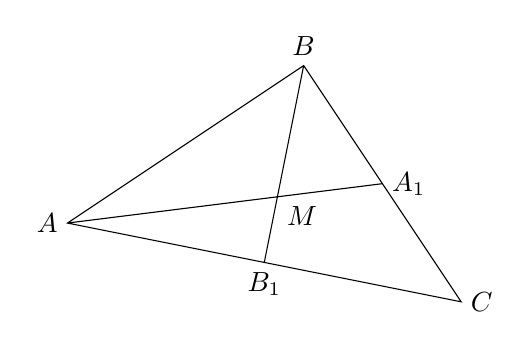
\begin{tikzpicture}
    \draw (0,1) coordinate[label=left:$A$] (A) --
    (3,3) coordinate[label=above:$B$] (B)  --
    (5,0) coordinate[label=right:$C$] (C) -- cycle
    (A) -- ($(B)!0.5!(C)$) coordinate[label=right:$A_1$](A1)
    (B)--($(A)!0.5!(C)$) coordinate[label=below:$B_1$](B1)
    (intersection cs:first line={(A)--(A1)},
    second line={(B)--(B1)}) coordinate[label=below right:$M$] (M);
  \end{tikzpicture}
  \caption{Środek masy trójkąta}
\end{figure*}
Dla układu n ciał środek masy to będzie ważona średnia położeń ciał. Zatem dla
układu n ciał o masach $m_i$ i położeniach $r_i$ środek masy to:

$$
M = \frac{\sum m_i \cdot r_i}{\sum m_i}
$$
oraz dla odległości od środka masy $d_i$ mamy $m_i \cdot d_i = d_n \cdot m_n$

\subsection{Zasada zachowania pędu}

$$
p = m \cdot v
$$
W izolowanym układzie pęd jest stały.

$$
p_{t=0} = p_{t=t}
$$

\subsection{Zderzenia}

Zderzenia to procesy w których ciała zmieniają swoje prędkości. Rozróżniamy
zderzenia sprężyste, w których energia kinetyczna jest zachowana, oraz
niesprężyste, w których energia kinetyczna nie jest zachowana.

\subsection{Popęd}

$$
J = \Delta p = F \cdot \Delta t
$$
Szczególnie przydatne jeśli np.: mamy wykres siły w czasie $F(t)$. Wtedy
$\int^{t_1}_{t_0} F(t) dt = \Delta p$

\section{Obroty}

\subsection{Bryła sztywna}

Bryła sztywna to ciało, które zachowuje swoją formę podczas ruchu. W odróżnieniu
od ciała punktowego, bryła sztywna ma rozmiar i kształt. Dla bryły sztywnej
mamy dwa rodzaje ruchu: ruch liniowy i ruch obrotowy.

\subsection{Przyspieszenie kątowe}

Zmiana kąta obrotu ciała to przyspieszenie kątowe. Jest to cecha całego ciała,
a nie jego składowych. Przyspieszenie kątowe to zmiana prędkości kątowej
w czasie.
\begin{figure*}[ht]
  \centering
  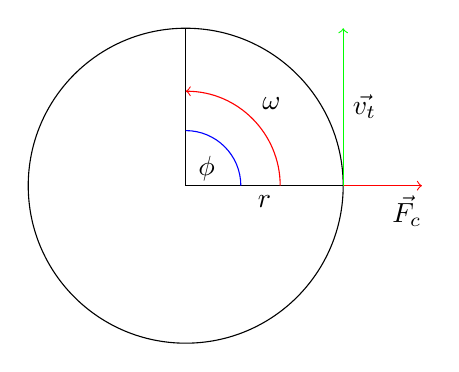
\begin{tikzpicture}
    \coordinate (O) at (0, 0);
    \coordinate (A) at (2, 0);
    \coordinate (A') at (0, 2);

    \draw (O) -- (A) node[midway, below] {$r$};
    \draw (O) -- (A');
    \draw[fill=none](0,0) circle (2.0);
    \draw[draw=blue] (O) ++(0:7mm) arc (0:90:7mm) node[midway, below
    left]{$\phi$};
    \draw[draw=red, ->] (A) -- (3, 0) node[midway, below right] {$\vec{F_c}$};
    \draw[draw=green, ->] (A) -- (2, 2) node[midway, right] {$\vec{v_t}$};
    \draw[draw=red, ->] (O) ++(0:1.2) arc (0:90:1.2) node[midway, above
    right]{$\omega$};
  \end{tikzpicture}
  \caption{Ilustracja wartości i sił w ruchu obrotowym}
\end{figure*}

$$
\omega = \frac{\Delta \phi}{\Delta t}, \quad \alpha = \frac{\Delta
\omega}{\Delta t}
$$
Prędkość kątowa jest analogiczna do prędkości liniowej, a przyspieszenie
kątowe do przyspieszenia liniowego.
$$
\int \alpha(t) dt = \omega(t)
$$

$$
\int \omega(t) dt = \phi(t)
$$

$$
\text{rpm} = \frac{2\pi}{60} \frac{\text{rad}}{\text{s}}
$$

\subsubsection{Punkt na obwodzie koła}
Prędkość punktu na obwodzie koła to prędkość styczna($v_t$). Dla koła mamy:
$$
\omega = \frac{v_t}{r}
$$
Punkt na obwodzie koła doświadcza przyspieszenia dośrodkowego:
$$
F_c = m \cdot a_c = m \cdot r \cdot \omega^2
$$
gdzie $a_c$ to przyspieszenie dośrodkowe, a $r$ to promień obrotu. Dla obiektu
o długości $l$ i jednorodnym rozłożeniu masy to $r = \frac{l}{2}$.

\subsection{Bezwładność, pęd i energia}

$$
I = \sum m_i r_i^2
$$
czyli suma momentów bezwładności wszystkich punktów materialnych w ciele.
Moment bezwładności wyraża opór ciała na zmianę ruchu obrotowego.
Dla pręta o długości $l$ mamy:
$$
I = \int r^2 dm
$$

\begin{table*}[ht]
  \centering
  \begin{tabular}{c|c}
    Ciało & Moment bezwładności \\ \hline
    Pręt & $I = \frac{1}{12} m \cdot l^2$ \\ \hline
    Koło & $I = \frac{1}{2} m \cdot r^2$ \\ \hline
    Pierścień & $I = m \cdot r^2$ \\ \hline
    Kula & $I = \frac{2}{5} m \cdot r^2$
  \end{tabular}
  \caption{Momenty bezwładności dla różnych ciał}
\end{table*}

Moment pędu:
$$
L = I \cdot \omega
$$

$$
W = \int^{\theta_0}_0 mgr\sin\theta d\theta = mgr(1 - \cos\theta_0)
$$

\subsection{Moment obrotowy (siły)}

$$
\tau = I \cdot \alpha = I \cdot \frac{\Delta \omega}{\Delta t} =
r\sin\alpha \cdot F = \frac{L}{\Delta t}
$$
gdzie $\alpha$ to kąt między siłą a promieniem obrotu.
O momencie obrotowym (torque) można myśleć jako o siły powodującej obrót
ciała. Aby zatrzymać obracające się ciało musimy zastosować siłę przeciwną
do momentu obrotowego. Jest to jakby siła odpowiedzialna za $\omega$.

$$
\vec{\tau} = \vec{r} \times \vec{F}
$$
gdzie $\vec{r}$ to pozycja a $\vec{F}$ to siła

\subsection{Twierdzenie Steinera}

W przypadku gdy znamy moment bezwładności względem jednej osi obrotu
(przechodzącej przez środek masy) to możemy obliczyć moment bezwładności
względem innej równoległej osi obrotu:
$$
I = I_0 + m \cdot d^2
$$

\subsection{Energia kinetyczna w ruchu obrotowym}

W jaki sposób obliczyć energię kinetyczną ciała w ruchu obrotowym? Wystarczy
zsumować energię kinetyczną wszystkich punktów materialnych w ciele.
Dla ciała które nie porusza się liniowo mamy:
$$
E_K = \sum \frac{1}{2} m_i v_{ti}^2 = \frac{1}{2} \sum m_i r_i^2 \omega^2 =
\frac{I\omega^2}{2}
$$
Dla ciała które porusza się liniowo i obrotowo mamy:
$$
E_K = \frac{m \cdot v^2}{2} + \frac{I \cdot \omega^2}{2}
$$
Dystrybucja energii na ruch obrotowy i postępowy zależy od momentu bezwładności.

\subsection{Porównanie ruchu liniowego i obrotowego}

\begin{table*}[ht]
  \centering
  \begin{tabular}{c|c|c}
    Cecha & Ruch liniowy & Ruch obrotowy \\ \hline
    przemieszczenie & $x$ & $\angle \theta$ \\ \hline
    prędkość & $v = \frac{\Delta v}{\Delta t}$ & $\omega =
    \frac{\Delta \theta}{\Delta t}$ \\ \hline
    przyspieszenie & $a = \frac{\Delta a}{\Delta t}$ & $\alpha =
    \frac{\Delta \omega}{\Delta t}$ \\ \hline
    bezwładność & $m$ & $I$ \\ \hline
    pęd & $p = m \cdot v$ & $L = I \cdot \omega$ \\ \hline
    zmiana pędu & $F = m \cdot a$ & $\tau = I \cdot \alpha$ \\ \hline
    $E_K$ & $\frac{m \cdot v^2}{2}$ & $\frac{I \cdot \omega^2}{2}$ \\ \hline
    Praca & $W = F \cdot d$ & $\tau \cdot \theta$
  \end{tabular}
  \caption{Porównanie ruchu liniowego i obrotowego}
\end{table*}

\section{Szczególna Teoria Względności}

Szczególna teoria względności to podzbiór ogólnej teorii względności, i nie
uwzględnia grawitacji. Skupia się na ruchu ciał w układach odniesienia
poruszających się z prędkościami zbliżonymi do prędkości światła.

Układ odniesienia obserwatora to zbiór elementów, które obserwator uważa za
spoczywające. Jeżeli prawa Newtona są prawdziwe w tym układzie, to jest to
inercjalny układ odniesienia. Na przykład: pokój to inercjalny układ
odniesienia, z kolei pociąg przyspieszający to nie jest inercjalny układ
odniesienia, ponieważ wewnątrz tego układu rzeczy postawione na ziemi będą
reagować na przyspieszenie.

Pomiędzy dwoma układami odniesienia poruszającymi się względem siebie
z niezerową prędkością, nie da się określić, który z nich jest w spoczynku dla
trzeciego obserwatora. W kontekście relatywistycznym nie ma absolutnego
spoczynku.

W mechanice klasycznej, czas jest absolutny i niezależny od układu odniesienia.
Zatem transformacja między dwoma układami odniesienia to po prostu przesunięcie
względem siebie. Pozycja $x$ w układzie $S$ ma postać $x' = x - ut$ w
układzie $S'$ i $t' = t$.

Jednym wielkim założeniem fizyki jako dziedziny, jest to że prawa fizyki są
takie same we wszystkich układach odniesienia. W szczególnej teorii względności
prawa fizyki są takie same we wszystkich inercjalnych układach odniesienia.
Jest to szczególnie istotne w kontekście czasu i odległości na skali w której
STW ma znaczenie.

\subsection{Postulaty}

\begin{enumerate}
  \item Wszyscy inercjalni obserwatorzy są równoważni.
  \item Prędkość światła w próżni jest stała i niezależna od prędkości
    źródła światła ani obserwatora.
\end{enumerate}

Z tych postulatów, oprócz nie możliwości osiągnięcia prędkości światła, wynika
to, że prawa są niezależne od prędkości obserwatora i są stałe.

\subsection{Transformacja Lorentza}

$$
\gamma = \frac{1}{\sqrt{1 - \frac{v^2}{c^2}}}
$$
Transformacja Lorentza to przekształcenie współrzędnych między układami
odniesienia poruszającymi się z różnymi prędkościami. Dla dwóch układów
odniesienia $S$ i $S'$ poruszających się względem siebie z prędkością $v$
względem siebie wzdłuż osi $x$ mamy:

$$
x' = \gamma(x - vt)
$$

$$
t' = \gamma(t - \frac{vx}{c^2})
$$
Relatywistyczna suma prędkości:
$$
u' = \frac{u + v}{1 - \frac{uv}{c^2}}
$$
Jeżeli układ $S'$ porusza się względem układu $S$ z prędkością $v$ i
w $S'$ ciało
ma prędkość $u$ to w układzie $S$ to ciało ma prędkość $u'$.

\begin{figure*}[h]
  \centering
  \begin{tikzpicture}[node distance=1cm]
    \node[draw, very thick, red] (x) at (-3,0.5) {$x$};
    \node[draw, very thick, above left=of x] (y) {$y$};
    \node[draw, very thick, above right=of x] (z) {$z$};
    \draw[->] (y.east) -- node[midway, above] {$v$} ++(1,0);
    \draw[->] (z.east) -- node[midway, above] {$u'$} ++(1,0);

    \draw[dotted] (0,0) -- (0,3) node[left] {$S$} node[right] {$S'$};

    \node[draw, very thick] (x) at (3, 0.5) {$x$};
    \node[draw, very thick, above left=of x, red] (y) {$y$};
    \node[draw, very thick, above right=of x] (z) {$z$};
    \draw[->] (z.east) -- node[midway, above] {$u$} ++(1,0);
    \draw[->] (x.west) -- node[midway, above] {$v$} ++(-1,0);
  \end{tikzpicture}
\end{figure*}

\subsection{Względność równoczesności}

Dla danego układu odniesienia zdarzenia odbywają się z różnicą czasu
$\le \Delta t_0$. Jest to stała dla danego układu odniesienia.
Dla obserwatora poruszającego się z prędkością $v$ zdarzenia
mogą odbywać się w różnych momentach czasu.

$$
\Delta t = \gamma \Delta t_0
$$

\subsection{Dylatacja czasu}

Dla obserwatora poruszającego się z prędkością $v$, dla obserwatora
poruszającego
się relatywnie wolniej, czas płynie szybciej i na odwrót.

$$
t = t_0 \cdot \gamma
$$

\subsection{Skrócenie długości}

Dla obserwatora w układzie odniesienia $S$ obserwator w układzie $S'$
poruszającym się z prędkością $v$ zauważy skrócenie długości ciała
w układzie $S$ i na odwrót.

$$
l = l_0 \cdot \gamma
$$
gdzie $l$ to długość ciała w układzie poruszającym się, a $l_0$ to długość
ciała w układzie stacjonarnym.

\subsection{Geometria czasoprzestrzeni}

W szczególnej teorii względności czas i przestrzeń są złączone w jedną
całość. Dlatego też zamiast mówić o czasie i przestrzeni mówimy o
czasoprzestrzeni.
Względność czasu i przestrzeni sprawia, że czas i przestrzeń są względne
i zależą od prędkości obserwatora. To oznacza, że pozycję w czasoprzestrzeni
wyraża się czterowektorem $(x, y, z, t)$.

\end{document}
